\newcommand{\blhat}{\widehat{\bloss}}
\newcommand{\bmu}{\boldsymbol{\mu}}
\newcommand{\bq}{\boldsymbol{q}}
\section{Wrapper Algorithm for Composite Losses}
\label{s:wrapper}
%
Our ``Composite Loss Wrapper'' algorithm (Algorithm~\ref{a:delayed-app}) wraps a standard bandit algorithm called here Base MAB (Base Multi-Armed Bandit). Base MAB operates on standard (noncomposite) losses with values in $[0,1]$,
producing probability distributions $\bp_t$ over the action set $\{1,\ldots,K\}$. The wrapper, which has access to a sequence
$B_0,B_1,\dots$ of i.i.d.\ Bernoulli random variables of parameter $q$ (to be chosen later), experiences three kinds of online rounds: a {\em draw}, an {\em update}, and a {\em stay}
round. If round $t$ is a draw round, the algorithm draws action $I_t$ according to the current distribution $\bp_t$
maintained by Base MAB, but without having Base MAB update $\bp_t$. If $t$ is an update round, then the algorithm's
action $I_t$ is the same as $I_{t-1}$ (in particular, the algorithm does not draw $I_t$ from $\bp_t$), but then a
distribution update $\bp_t \rightarrow \bp_{t+1}$ takes place by invoking the update rule of Base MAB over an
average of the observed losses.
Finally, if $t$ is a stay round, then both $I_t = I_{t-1}$ and $\bp_{t+1} = \bp_{t}$. The way these three
kinds of rounds are interleaved is illustrated in Figure~\ref{f:1}.
%
%% ----------------------------------------------------------------------------
\begin{algorithm2e}[t]
\SetKwSty{textrm} \SetKwFor{For}{{\bf For}}{}{}
\SetKwIF{If}{ElseIf}{Else}{if}{}{else if}{else}{}
\SetKwFor{While}{while}{}{}
\textbf{Input:}  Base MAB algorithm $A$ with parameter $\eta \in (0,1]$.\\%, and meta-parameters for it $\xi$.\\
\textbf{Initialize:}
\begin{itemize}[topsep=0pt,parsep=0pt,itemsep=0pt]
\item Draw $I_0$ from the uniform distribution $\bp_1$ over $\{1,\ldots,K\}$;
\item If $B_0 = 1$ then $t=0$ is an update round.
\end{itemize}
%
\For{$t=1,2,\dots$:} { {
\begin{enumerate}[topsep=0pt,parsep=0pt,itemsep=0pt]
\item If $t-1$ was an update round, then draw $I_t \sim \bp_t$ and play it without updating $\bp_t$ (draw round, $\bp_{t+1} = \bp_t$);
\item Else if an update round was in the interval $\{t-2d+1, \dots,t-2\}$ then play $I_t = I_{t-1}$ without updating $\bp_t$
(stay round, $\bp_{t+1} = \bp_t$);
\item Else play $I_t = I_{t-1}$ (stay round), and if $B_t=1$ then the stay round becomes an update round. In such a case:
%
\begin{minipage}{\textwidth-50pt}
\begin{itemize}
\vspace{0.05in}
\item Feed Base MAB $A(\eta)$ with average composite loss\footnote
{
Recall that when $t \leq 0$, we defined $\ell^{(s)}_{t} =0$, so the initial stretch of $2d-2$ actions $I_1,\ldots,I_{2d-2}$ can be disregarded here at the price of an extra additive $\scO(d)$ regret in the analysis.
}
%
\[
\avgloss_t = \frac{1}{2d}\sum_{\tau=t-d+1}^t \lcomp_\tau(I_{\tau-d+1},\dots,I_{\tau})
\]
\item Use the update rule $\bp_t\rightarrow \bp_{t+1}$ of Base MAB to obtain the new distribution $\bp_{t+1}$.
%(the stay round becomes an update round).
\end{itemize}
\end{minipage}
\end{enumerate}
%\vspace{-0.2in}
} } \caption{The Composite Loss Wrapper.}
\label{a:delayed-app}
\end{algorithm2e}
%% ---------------------------------------------------------------------------
%
\begin{figure}[t!]
\begin{picture}(-40,290)(-40,290)
\scalebox{0.7}{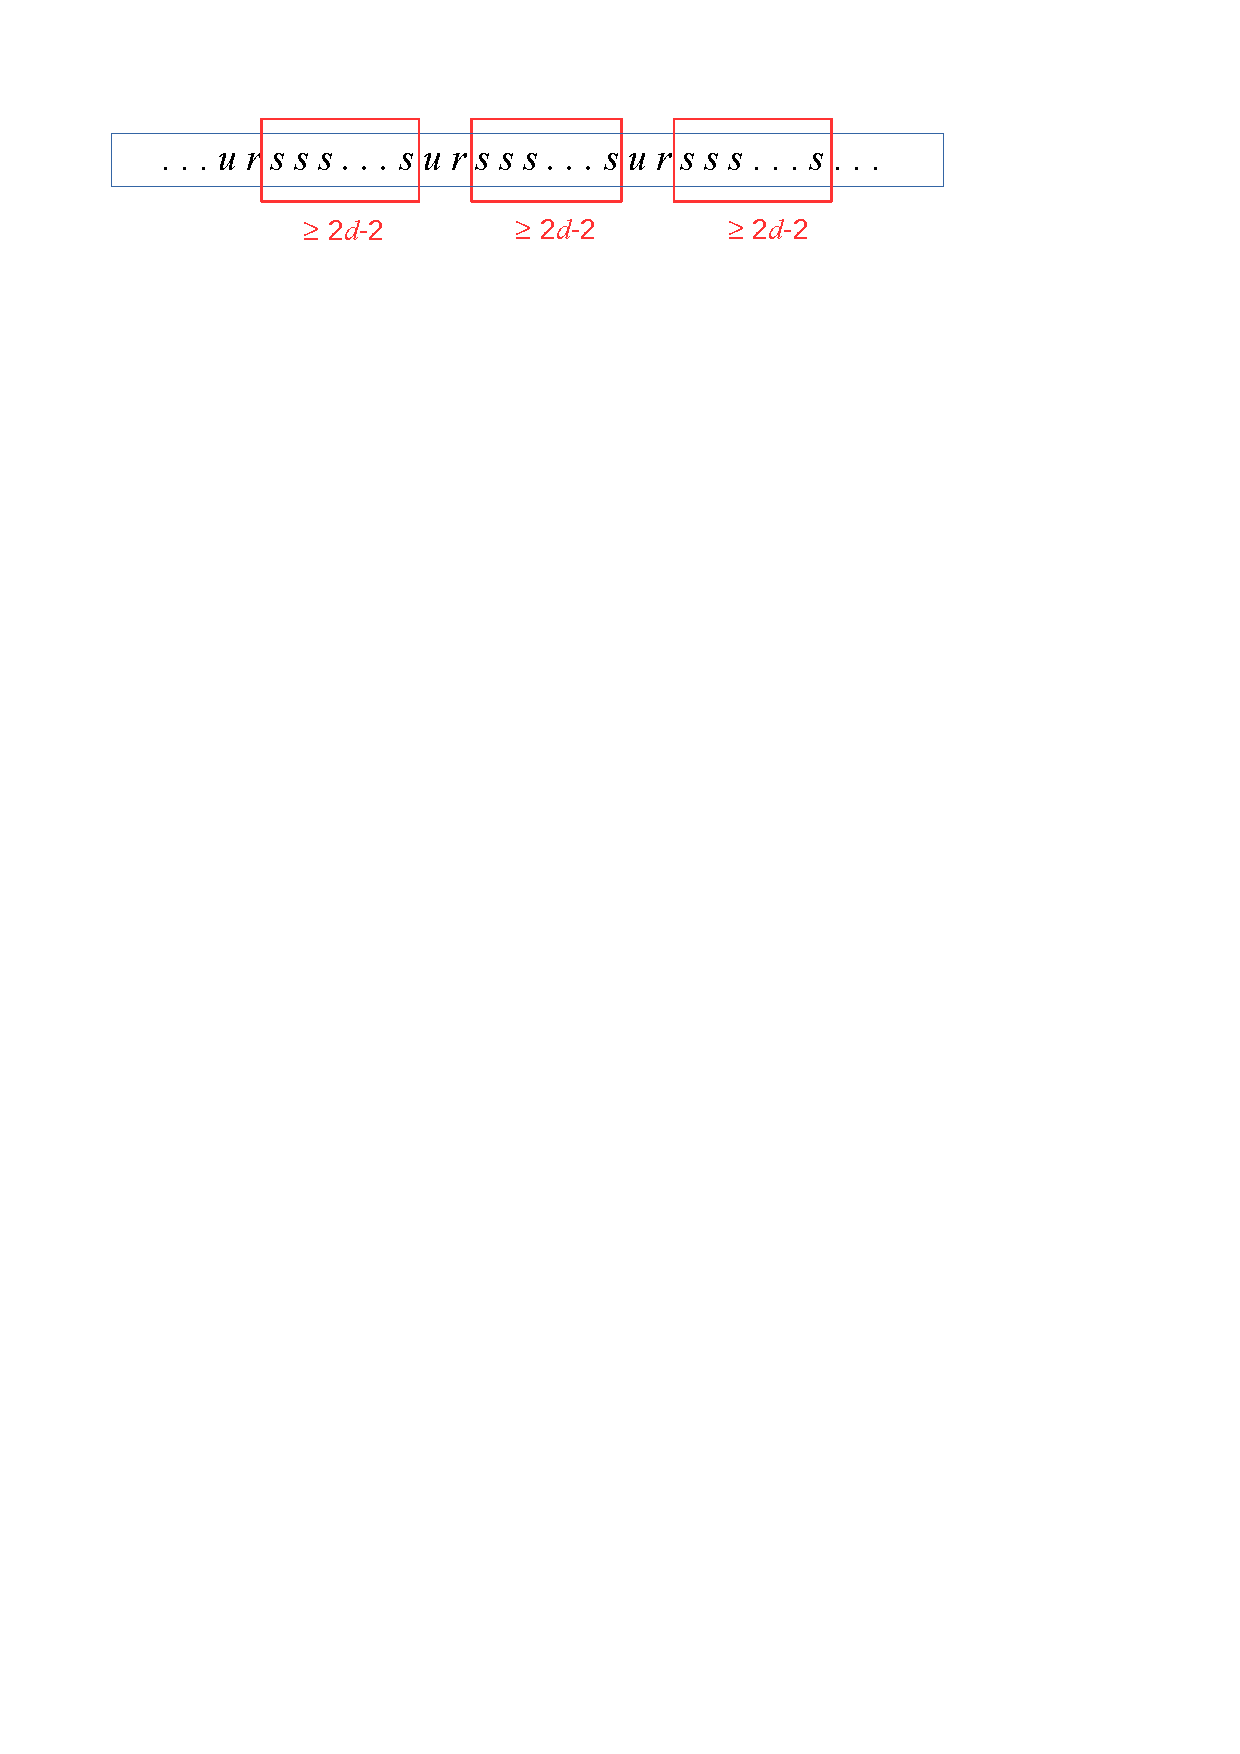
\includegraphics{interleave.pdf}}
\end{picture}
\vspace{-3.0in}
\caption{\label{f:1}
Sequence of rounds the algorithm is undergoing. Each ({\em u})pdate round is always followed by a d({\em r})aw round,
and then by a stretch of ({\em s})tay rounds whose length is random, but is at least $2d-2$.
The actual length of the stay stretch is ruled by the realizations of the Bernoulli random variables $B_t$.
}
\end{figure}


%%% ----------------------------------------------------------------------------
%\begin{algorithm2e}[t]
%\SetKwSty{textrm} \SetKwFor{For}{{\bf For}}{}{}
%\SetKwIF{If}{ElseIf}{Else}{if}{}{else if}{else}{}
%\SetKwFor{While}{while}{}{}
%\textbf{Parameter:} $\eta \in [0,1]$.\\
%\textbf{Initialize:}
%\begin{itemize}
%\item Draw $I_0$ from the uniform distribution $p_1$;
%\item If $B_0 = 1$ then $t=0$ is an update round.
%\end{itemize}
%%
%\For{$t=1,2,\dots$:}
%{ {
%\begin{enumerate}
%\item If $t-1$ was an update round, then draw $I_t \sim p_t$ and play it without updating $p_t$ (draw round);
%\item Else if $d > 2$ and an update round was in the interval $\{t-d+1, \dots,t-2\}$ then play $I_t = I_{t-1}$ without updating $p_t$
%(stay round);
%\item Else play $I_t = I_{t-1}$ (stay round), and if $B_t=1$ then perform an Exp3$(\eta)$ update of $p_t$
%using $\loss_t(I_t,\dots,I_{t-d+1})$ (the stay round becomes an update
%round).
%\end{enumerate}
%
%\vspace{-0.2in}
%} }
%\caption{Delayed Loss Algorithm}
%\label{a:delayed}
%\end{algorithm2e}
%%% ----------------------------------------------------------------------------
%%
%
Note that the algorithm's pseudocode corresponds to the description in Figure~\ref{f:1} in that update and draw rounds are interleaved,
and an update round is immediately followed by a draw round. If an update round occurs at time $t \ge 1$, then no update round
can occur during the next $2d-1$ rounds; the next update takes place at time $t+2d+G$ where $G \ge 0$ is a Geometric random variable
with parameter $q$. Hence a stretch of stay rounds is $2d-2+G$ round long.
Moreover,
\begin{itemize}[topsep=0pt,parsep=0pt,itemsep=0pt]
\item
If $t$ is not a draw round (i.e., it is either an update or a stay round), then the last action is played again.
\item
If $t$ is an update round, then we are guaranteed that $I_t=\cdots=I_{t-2d+1}$, since the last draw could have only occurred
at time $t-2d+1$ or earlier.
\end{itemize}
%
In order for our analysis to go through, we make mild assumptions on Base MAB. The first assumption (fulfilled by many
standard $K$-armed bandit algorithms ---see below) is a stability condition described in the following definition.
%
\begin{definition}\label{d:stabilityexp3}
Let $A(\eta)$ be a Base MAB with learning rate $\eta$,
and $\{\bp_t\}_{t=1}^T$ be the sequence of probability distributions over actions $\{1,\ldots,K\}$ produced by $A(\eta)$ during a run over $T$ rounds. We say that $A(\eta)$ is $\xi$-{\em stable} if for any round $t$ we have that
\[
    \E\left[\sum_{i\,:\,p_{t+1}(i) > p_t(i)} p_{t+1}(i) - p_t(i)\right] \leq \xi
\]
% deterministically
holds, where $\xi = \xi(K,\eta,\ldots)$ is a function of $K$, $\eta$, and possibly other relevant parameters of the Base MAB.
\end{definition}
%
The second assumption is that $A(\eta)$ is {\em nontrivial} for any $\eta > 0$:
when operating in the standard (non-delayed) bandit setting, $A(\eta)$ enjoys a concave (possibly linear) regret bound as a function of the time
horizon $T$.  Specifically, if we let $R_A(T,K,\eta)$ be a regret bound for $A$ when the time horizon is $T$, the number
of actions is $K$ and the learning rate is $\eta$, we have for any $K \geq 1$ and $\eta > 0$ that
%$R_A(T,K,\eta) = o(T)$ as $T \rightarrow \infty$, being
$R_A(T,K,\eta)$ is a concave function of $T$. For example,
$R_A(T,K,\eta) = \scO((\ln K)/\eta + \eta K T)$, which is linear in
$T$.
%
\iffalse
*********************************
Our algorithm receives a general Multi-Arm Bandit algorithm $A$,
which has a learning rate parameter $\eta$ and a set of hyper
parameters $\xi$. We will assume that MAB is {\em stable}, namely,
it does not change the action distribution by more than $2\eta$
between successive rounds. Formally, the definition of stable is the
following.
%
\begin{definition}
A MAB algorithm $A$ with parameter $\eta$ is {\em stable} if for any
history $h$ and loss $\ell$: it outputs the distribution $p$ after
$h$ and the distribution $p'$ after $h$ followed by $\ell$, then
$\|p-p'\|_1\leq 2\eta$
\end{definition}
%
The regret bound of a MAB algorithm $A$ with parameters $\eta$ and
$\xi$ is denoted by $R_A(T,K,\eta,\xi)$. Namely, for any sequence of
losses $\ell_t$ and any fixed action $j$ we have,
\[
\E[\sum_{t=1}^T \ell_t(a_t)]\leq \E[\sum_{t=1}^T \ell_t(j)] + R_A(T,K,\eta,\xi)
\]
where the expectation is over the probabilities that $A$ selects
action $a_t$ at time $t$.

We also assume that for any random variable ${\cal T}$ we have
\[
\E[R_A({\cal T},K,\eta,\xi)]\leq R_A(\E{\cal T},K,\eta,\xi)
\]
*********************************
\fi
We have the following theorem, whose proof is in the appendix.
%
\begin{theorem}\label{thm:delay-generic}
Let $A(\eta)$ be a $\xi$-stable and nontrivial Base MAB algorithm with learning rate $\eta$ and regret bound
$R_A(T,K,\eta)$ for standard $K$-armed bandits. Then
Algorithm~\ref{a:delayed-app} with input $A(\eta)$ achieves regret
\[
R_T \le T\,\xi + 8(2d-1)R_A(T/2d,K,\eta) + \scO(d)
\]
for $K$-armed bandits with $d$-delayed composite anonymous feedback.
%In particular, for $\eta = \sqrt{\frac{d\ln K}{TK}}$ we have a
%cumulative regret of $O(\sqrt{dTK\ln K} )$
\end{theorem}
%
%
%%%%%%%%%%%%%%%%%%%%%%%%%%%%%%%
%
We can now derive corollaries for various algorithms using Theorem~\ref{thm:delay-generic}. Consider for instance, the well-known
Exp3 algorithm of \citet{AuerCeFrSc02}. When operating with losses, the algorithm maintains a probability distribution
$\bp_t = (p_t(1),\ldots,p_t(K))$ over $\{1,\ldots,K\}$ of the form $p_t(i) = w_t(i)/\sum_{j=1}^K w_t(j)$, while the update rule
$\bp_t\rightarrow \bp_{t+1} $ can be described as follows:
\begin{equation}
\label{eq:expW}
w_{t+1}(i) = p_t(i)\,e^{-\eta\ellhat_t(i)},\quad \ellhat_t(i) = \frac{\ell_t(i)\Ind{I_t = i}}{p_t(i)},\quad i = 1, \ldots, K~.
\end{equation}
When the losses $\ell_t(i)$ are in $[0,1]$ we have the regret bound
\(
R_{\mathrm{Exp3}}(T,K,\eta) \leq \frac{\ln K}{\eta}+\frac{\eta}{2}\,K\,T~.
\)
Moreover, the following simple stability property holds (proof in the appendix).
%
\begin{lemma}\label{l:stabilityexp3}
Exp3 with learning rate $\eta$ is $\xi$-stable with $\xi = \eta$.
\end{lemma}
%
Combined with Theorem~\ref{thm:delay-generic}, this implies the following regret bound with composite losses.
%
\sloppypar{
\begin{corollary}\label{c:delay-generic}
%With the notation introduced so far,
If Algorithm~\ref{a:delayed-app} is run with Exp3($\eta$) with $\eta = 4\sqrt{\frac{d\,\ln K}{(4K+1)\,T}}$ as Base MAB, then its regret for $K$-armed bandits with $d$-delayed composite anonymous feedback satisfies
\[
R_T \leq 8\sqrt{d\,(4K+1)\,T\,\ln K} + \scO(d) = \scO(\sqrt{dKT\ln K})~.
\]
\end{corollary}
}
%
$K$-armed bandits are a special case of combinatorial linear bandits
\citep{cesa2012combinatorial}, a setting where actions are incidence
vectors $\bv\in\scK\subset\bool^n$ describing elements in some
combinatorial space (e.g., spanning trees of a given graph) and loss
vectors $\bloss_t \in [0,1]^n$ satisfy $\bloss_t^{\top}\bv \in
[0,1]$ for all $\bv\in\scK$ (in $K$-armed bandits, $\scK$ is simply
the canonical basis of $\bool^n$). Let $\bv_t\in\scK$ be the action
played at time $t$. The generalization of Exp3 for the combinatorial
bandit setting uses the Exp2 algorithm with loss estimates of the
form $\blhat_t = P_t^+ \bv_t \bv_t^{\top} \bloss_t$, where $P_t =
\E_{\bV \sim \bp_t}\bigl[\bV \bV^{\top}\bigr]$ and $P_t^+$ is the
pseudo inverse of $P_t$ ---see \citep{dani2008price}. Note that
these estimates are unbiased: $\E_t\big[\blhat_t^{\top}\bv] =
\bloss_t^{\top}\bv$ for all $\bv\in\scK$. The distribution $\bp_t$
is a mixture $\bp_t = (1-\gamma)\bq_t + \bmu$, where $0 < \gamma <
1$, $\bq_t$ has the exponential form~(\ref{eq:expW})
\[
    q_t(\bv) = \frac{w_t(\bv)}{\sum_{\bv'\in\scK} w_t(\bv')}~,
\quad
    w_{t+1}(\bv)
=
    q_t(\bv)\,e^{-\eta\,\blhat_t^{\top}\bv}~,
\quad
    \bv\in\scK~,
\]
and $\bmu$ is a fixed exploration distribution on $\scK$. When run with an appropriate exploration distribution $\bmu$ and $\gamma = \eta n < 1$, Exp2$(\eta)$ has the following regret bound ---see, e.g., \citep[Theorem~4]{bubeck2012towards},
$
    R_{\mathrm{Exp2}}(T,\scK,\eta) \le \big(\ln|\scK|\big)\big/{\eta} + 3\eta nT
$.
Now, similarly to Lemma~\ref{l:stabilityexp3}, we can prove the following (the proof is provided in the appendix):
%
\begin{lemma}
\label{l:stabExp2}
Exp2 with learning rate $\eta$ and mixing coefficient $\gamma$ is $\xi$-stable with $\xi = (1-\gamma)\eta$.
\end{lemma}
%
Combining again with Theorem~\ref{thm:delay-generic}, the above implies the following regret bound with composite losses.
%
\begin{corollary}
\label{c:delayExp2}
If Algorithm~\ref{a:delayed-app} is run with Exp2($\eta$) with $\eta = 4\sqrt{\frac{d\,\ln|\scK|}{(24n+1)\,T}}$ as Base MAB, then its regret for $\scK$-combinatorial bandits, $\scK \subseteq \{0,1\}^n$, with $d$-delayed composite anonymous feedback satisfies
\[
    R_T
\le
    8\sqrt{d\,(24n+1)\,T\,\ln|\scK|} + \scO(d) = \scO(\sqrt{dnT\ln|\scK|})~.
\]
\end{corollary}
%
\begin{remark}\label{r:firstorderbound}
The proof of Lemma~\ref{l:stabilityexp3} in the appendix shows pointwise stability, a stronger notion than the expected stability of Definition~\ref{d:stabilityexp3}. In fact, an outer expectation over the random variable $I_t$ in the proof of Lemma~\ref{l:stabilityexp3} makes the stability parameter $\xi$ be upper bounded by $\eta\sum_{i=1}^K p_{t}(i)\ell_{t}(i)$ in round $t$, so that the term $T\xi$ in Theorem~\ref{thm:delay-generic} can be replaced by $\eta\,L_A(T)$, where $L_A(T)$ is the cumulative (average) loss of the Base MAB. Coupled with a ``first order" regret analysis of Exp3 where $T$ is indeed replaced by $L_A(T)$ ---see~\citep[Theorem~2]{allenberg2006hannan}, this gives a regret bound in the composite anonymous feedback setting where $T$ is likewise replaced by $L_A(T)$.
\end{remark}
